\chapter{Monte Carlo Methods}
\label{cha:Monte Carlo Methods}

As shown in the last chapter, Bayesian model comparison in practice usually
involves computations of some integrations with respect to complex posterior
distributions. Only in very special situations, these can be resolved
analytically. In most cases, these integrations are approximated using
simulation techniques.

\section{Classical Monte Carlo}
\label{sec:Classical Monte Carlo}

Classical Monte Carlo integration approximates the expectation of a function
$\varphi$ with respect to a distribution $\pi$,
\begin{equation}
  \Exp_{\pi}[\varphi(X)] = \int\varphi(x)\pi(x)\intd x
\end{equation}
provided that the above expectation exists, by drawing \iid samples from
$\pi$, say $\{X^{(i)}\}_{i=1}^N$, and approximating the expectation by the
empirical average,
\begin{equation}
  \hat\varphi^N = \frac{1}{N}\sum_{i=1}^N\varphi(x^{(i)}).
  \label{eq:vanilla mc}
\end{equation}
This method is sometime also called \emph{vanilla} Monte Carlo or \emph{naive}
Monte Carlo.

The estimator $\hat\varphi^N$ converges almost surely to
$\Exp_{\pi}[\varphi(X)]$ when $N\to\infty$ by the Strong Law of Large Numbers
(\slln). The variance of the estimator,
\begin{equation}
  \var_{\pi}[\hat\varphi^N] =
  \frac{1}{N} \int (\varphi(x) - \Exp_{\pi}[\varphi(X)])^2 \pi(x) \intd x
\end{equation}
can also estimated by
\begin{equation}
  \hat{V}^N = \widehat{\var_{\pi}[\hat\varphi^N]} =
  \frac{1}{N^2} \sum_{i=1}^N (\varphi(x^{(i)}) - \hat\varphi^N)^2
\end{equation}
provided that $\varphi^2$ has a finite expectation under $\pi$. In addition,
confidence bounds on the estimator can also be constructed, since the central
limit theorem (\clt) ensures that,
\begin{equation}
  \lim_{N\to\infty} \sqrt{N} (\hat\varphi^N - \Exp_{\pi}(\varphi(X)))
  \xrightarrow{D} \calN(0, \var_{\pi}[\varphi(X)]
\end{equation}
and thus for large $N$,
\begin{equation}
  \frac{\hat\varphi^N - \Exp_{\pi}[\varphi(X)]}{\sqrt{\hat{V}^N}}
\end{equation}
is approximately distributed as a $\calN(0, 1)$ random variable where
$\calN(\mu,\sigma^2)$ denotes the Normal distribution with mean $\mu$ and
variance $\sigma^2$ \cite[][sec.~3.2]{Robert:2004tn}.

Clearly this method can only be applied when drawing samples directly from the
target distribution $\pi$ is possible. There are a few ways to draw random
variates from an arbitrary distribution. See \cite[][chap.~2]{Robert:2004tn}
on this topic. In many cases, simulation from a distribution $\pi$ efficiently
requires the evaluations of its density function point-wise, or finding some
easy to simulation distribution that closely imitate $\pi$. In the context of
Bayesian computation, the target distributions are usually complex posterior
only known up to some normalizing constants. And thus point-wise evaluation is
not possible. In addition, the high-dimensional aspects of many models makes
it near impossible to find a distribution closely imitate the target.

In the particular context of Bayesian model comparison, it is often difficult
to use vanilla Monte Carlo integration. For example, consider the
approximation of the marginal likelihood, which is required to evaluate the
Bayes factor (section~\ref{sub:Bayes factor}),
\begin{equation*}
  p(\data|\calM_k) =
  \int f(\data|\theta_k,\calM_k)\pi(\theta_k|\calM_k) \intd \theta_k.
\end{equation*}
It might appears to be possible to express it as
\begin{equation}
  p(\data|\calM_k) = \Exp_{\pi}[f(\data|\theta_k,\calM_k)],
  \label{eq:prior expectation}
\end{equation}
and use samples from $\pi(\theta_k|\calM_k)$, the prior distribution, to
approximate the integration. However, such approaches often results in large
variance since simulating from the prior distribution can results in a large
proportions of samples having small likelihood. In other words, the likelihood
function (and thus the posterior distribution) is often much more concentrated
than the prior distribution. For instance, considering the \pet model with one
component and a informative prior. Using 100,000 samples from the prior
distribution, the empirical mean and standard deviation of the estimates from
100 simulations is $-40.9$ and $2.1$, respectively. However when the dimension
of the model is increased by using a two components, the estimates have a
empirical mean and variance $-39.6$ and $12.6$, respectively, which is too
large a variance for practice use of evaluating the Bayes factor. In general,
the variance of a vanilla Monte Carlo estimator is influenced by both the
function $\varphi$ and the distribution $\pi$.

\section{Importance sampling}
\label{sec:Importance sampling}

The \emph{importance sampling} method is based on the identity, termed
\emph{importance fundamental identity} by \cite{Robert:2004tn},
\begin{equation}
  \Exp_{\pi}[\varphi(X)]
  = \int\varphi(x)\pi(x)\intd x
  = \int\varphi(x)\frac{\pi(x)}{\eta(x)}\eta(x)\intd x
  = \Exp_{\eta}\Square[Big]{\varphi(X)\frac{\pi(X)}{\eta(X)}},
\end{equation}
where $\eta$ is a distribution with respect to which $\pi$ is absolutely
continuous. This distribution is often called the \emph{proposal} or
\emph{instrumental} distribution. Thus given \iid samples
$\{X^{(i)}\}_{i=1}^N$ from distribution $\eta$, the expectation
$\Exp_{\pi}[\varphi(X)]$ can be approximated by the following importance
sampling estimator,
\begin{equation}
  \hat\varphi_{\is}^N
  = \frac{1}{N}\sum_{i=1}^N\varphi(X^{(i)})\frac{\pi(X^{(i)})}{\eta(X^{(i)})}.
  \label{eq:is normalized}
\end{equation}
The above estimator also converges almost surely to $\Exp_{\pi}[\varphi(X)]$
when $N\to\infty$. However its variance is not necessarily finite. In general
the variance is finite if and only if,
\cite[][sec.~3.3.2]{Robert:2004tn},
\begin{equation}
  \int(\varphi(x))^2\frac{(\pi(x))^2}{\eta(x)} < \infty.
\end{equation}
This suggests that the density $\eta$ shall have tails heavier than those of
$\pi$. To access the above inequality, evaluating of a more complex
integration than the original problem is required. Some rather restrictive
sufficient conditions for finite variance estimator was mentioned in
\cite{Geweke:1989tm}. It is sufficient to mention here that most conditions
that guarantee the variance of $\hat\varphi_{\is}$ being finite
or optimal requires knowledge of $\pi$ that is not available. And thus they
are not of particular interest for practical interest.

In practice both $\pi$ and $\eta$ are often only known up to some normalizing
constants, which can be approximated with the same samples. This leads to the
estimator,
\begin{equation}
  \hat\varphi_{w\is}^N
  = \frac{\sum_{i=1}^Nw^{(i)}\varphi(X^{(i)})}{\sum_{i=1}^Nw^{(i)}}
  \label{eq:is unnormalized}
\end{equation}
where $w^{(i)} \propto \pi(X^{(i)})/\eta(X^{(i)})$, and is termed the
\emph{weights}. This estimator also converges almost surely to
$\Exp_{\pi}[\varphi(X)]$ when $N\to\infty$. This estimator has a small
bias since it is the ratio of two unbiased estimator. However, even when the
normalizing constants of $\pi$ and $\eta$ are both known, this estimator can
be preferable to $\hat\varphi_{\is}$ due to its possible improvement in the
squared mean of errors. In fact, \cite{Casella:1998tj} showed an example of
using the Cauchy distribution as the proposal distribution for the evaluation
of expectations under the Student-$t$ distribution, where for some
functions, such as $\varphi(x) = |x|$, $\hat\varphi_{w\is}$ can
outperform $\hat\varphi_{\is}$ considerably.

In general, similar to vanilla Monte Carlo, the performance of importance
sampling depends not only on the choice of the proposal distribution $\eta$,
but also the function of interest $\varphi$. As suggested in
\cite[][sec.~3.3.2]{Robert:2004tn}, to minimize the variance of the estimator,
the distribution $\eta$ should be chosen such that
$|\varphi(x)|\pi(x)/\eta(x)$ is almost constant with a finite variance. That
is, it is preferable for the distribution $\eta$ to be proportional to
$|\varphi|\pi$ and have heavier tails. In practice, often the same samples are
used to evaluate the expectations of different functions. And the proposal
distribution is chosen such that $\eta$ is close to $\pi$ with a heavier tail.

In Bayesian modeling, if we are interested in the evaluation of the marginal
likelihood function for the purpose of model comparison, and use the
expression~\ref{eq:prior expectation}, then the above guidelines require the
knowledge of $f(\data|\theta_k,\calM_k)\pi(\theta_k|\calM_k)$, which is hardly
available. If we are interested in evaluations of expectations of various
functions under the posterior distributions, such as the posterior mean of
parameters, and attempt to a distribution close to the posterior distribution
as the proposal distribution, then we face the same difficulty.

In the next chapter, we will see that, it is possible to construct efficient
proposal distributions iteratively.

\section{Markov chain Monte Carlo}
\label{sec:Markov chain Monte Carlo}

Both the vanilla Monte Carlo and importance sampling methods require
simulations directly from a distribution, which is often not feasible in
realistic applications. Especially for the purpose of Bayesian modeling, the
target is often a complex posterior distribution. Estimation techniques based
on dependent samples were developed. The most important type, Markov chain
Monte Carlo (\mcmc), uses dependent samples generated by a Markov chain with
the target $\pi$ as a limiting distribution for the approximation of the
desired integration. A limiting distribution, informally is one such that if
$X_n$, the state of the Markov chain at step $n$ is distributed with $\pi$,
then $X_{n+1}$, the next step is also distributed with $\pi$.

The basic idea is that, given a Markov chain $(X^{(1)},\dots,X^{(i)},\dots)$,
with a limiting distribution $\pi$, then with suitable conditions (outlined
for each algorithm later), for a $\pi$-integrable function $\varphi$,
\begin{equation}
  \lim_{N\to\infty}\frac{1}{N}\sum_{i=1}^N\varphi(X^{(i)}) =
  \Exp_{\pi}[\varphi(X)]
  \label{eq:mcmc convergence}
\end{equation}
And therefore samples generated by this Markov chain can be used for
estimation of various quantities in a similar fashion as with vanilla Monte
Carlo or importance sampling. This leads to the estimator,
\begin{equation}
  \hat\varphi_{\mcmc}^N = \frac{1}{N}\sum_{i=1}^N\varphi(X^{(i)})
  \label{eq:mcmc est}
\end{equation}
where $\{X^{(i)}\}_{i=1}^N$ are $N$ samples from the Markov chain.

The construction of such a $\pi$-invariant Markov kernel leads to development
of various widely used \mcmc algorithms. In this section, some of the most
important ones are reviewed.

\subsection{Discrete time Markov chain}
\label{sub:Discrete time Markov chain}

This section briefly reviews some notions of discrete time Markov chains. Due
to its utility natural, it will be compact and only reviews results required
by later sections.

A Markov chain can be defined in terms of \emph{transition kernels}. Consider
a measurable space, say $(E,\calE)$, a transition kernel $K$ is a function defined
on $E\times\calE$ such that $K(x,\cdot)$ is a probability measure for every
$x\in E$ and $K(\cdot,A)$ is measurable for every $A\in\calE$. In the
continuous case, we also call the corresponding conditional density
\emph{kernel}, denoted by $K(x,x')$, $x,x'\in E$. That is, $\Pr(X\in A|x) =
\int_A K(x,x')\intd x'$.

A (discrete time) Markov chain, denoted by $(X_n)$ is a sequence of random
variables $X_0,X_1,\dots,X_n,\dots$ such that conditional on
$x_{n-1},\dots,x_0$, $X_n$ has the same distribution as it has conditional on
$X_{n-1}$. Clearly a transition kernel $K(x_{n-1},\diff x_n)$ is such a
conditional distribution. In the context of \mcmc, we are mostly concerned
with \emph{time homogeneous} Markov chains. A Markov chain $(X_n)$ is said to
be time homogeneous if for every $t_0\le t_1\le\dots\le t_k$, the distribution
of $(X_{t_1},\dots,X_{t_k})$ conditional on $x_{t_0}$ is the same as
$(X_{t_1-t_0},\dots,X_{t_k-t_0})$ conditional on $x_0$. In other words, given
the initial state $x_0$ or its distribution, the Markov chain is determined
solely by its transition kernel.

Another way to define a Markov chain, or its defining property is the
\emph{(weak) Markov property}: For every initial distribution of $X_0$, $\mu$,
and every $(n+1)$ sample $(X_0,\dots,X_n)$,
\begin{equation}
  \Exp_{\mu}[\varphi(X_{n+1},X_{n+2},\dots)|x_0,\dots,x_n] =
  \Exp_{x_n}[\varphi(X_1,X_2,\dots)],
\end{equation}
where $\Exp_{\mu}$ denotes the expectation with respect to $P_{\mu} = \mu
K^n$, $K^n = K\vysmwhtcircle K^{n-1}$ and $\varphi$ is a $P_{\mu}$-integrable
function.

We will be mostly concerned with the sensitivity of the Markov chain with
respect to the initial value $X_0$ or its distribution and the existence and
the speed at which the Markov chain converges to its limiting distribution. A
few properties of a given Markov chain are discussed below. In short,
\emph{irreducibility} states that all states communicate. The Markov chain can
reach any state $y\in E$ starting from any other state $x\in E$. A stronger
version says that the chain can travel any distance in one step. A somewhat
opposite property is \emph{aperiodic}, which in essence says that a Markov
chain can stay in the neighborhood for an arbitrary number of instances. Or it
does not need to go through a cycle to reach back into the neighborhood of the
current state. These two properties guarantee a Markov chain to explore a
space freely. A third property we will discuss is \emph{recurrence}, which
states that the Markov chain can visit any state for infinite times. In other
words, the Markov chain can explore a space throughout starting from almost
anywhere. A stronger version, \emph{Harris recurrence}, allows the chain to
start from \emph{everywhere}. A property fundamental to \mcmc algorithms is
the existence of \emph{invariant} distribution, which states that the Markov
chain can be stable under suitable conditions and converge to a desired
distribution. A sufficient condition for the existence of invariant
distribution, \emph{detailed balance}, is perhaps the most useful tool in
practice to check the validity of a given algorithm. Last, we will discuss the
\emph{ergodicity} of Markov chains, which measures the speed at which a Markov
chain converges to its invariant (and thus its limiting) distribution.

In what follows, we give a more formal yet compact treatment of the properties
discussed above. Most results are stated without proofs. One can see, for
example \cite[][chap.~6]{Robert:2004tn} for a treatment of the topic in more
detail in the context of \mcmc algorithms.

\subsubsection{Irreducibility}

A Markov chain $(X_n)$ with transition kernel $K$ on $(E,\calE)$ is said to be
$\psi$-\emph{irreducible}, for a given measure $\psi$, if for every
$A\in\calE$ with $\psi(A)>0$, there exists $n$ such that $K^n(x,A)>0$ for all
$x\in E$. This chain is said to be \emph{strongly} $\psi$-\emph{irreducible}
if $n=1$ for all measurable $A\in\calE$.

An equivalent way of saying irreducibility is that for $x\in E$, $A\in\calE$,
$P_x(\tau_A\le\infty) > 0$, where $\tau_A = \inf\{n\ge1;X_n\in A\}$ is the
first value of $n$ that the chain enters the set $A$, namely the
\emph{stopping time} at $A$ and $P_x$ denote the probability conditional on
initial state $x$. In other words, the probability of reach the set $A$ in
finite steps is positive.

Two related concepts are \emph{atom} and \emph{small set}. A Markov chain
$(X_n)$ is said to have an \emph{atom} $\alpha\in\calE$  if there exits an
associated nonzero measure $\eta$ such that, $K(x,A) = \eta(A)$ for all
$x\in\alpha$ and $A\in\calE$. A set $C$ is said to be \emph{small} if there
exits $m\in\Natural$ and a nonzero measure $\eta_m$ such that
$K^m(x,A)\ge\eta_m(A)$, for all $x\in C$ and $A\in\calE$.

A result that relates small set and irreducibility is that, for a
$\psi$-irreducible chain $(X_n)$, and for all $A\in\calE$ such that
$\pi(A)>0$, there exists $m\in\Natural$ and a small set $C\subset A$ such that
the associated measure $\eta_m$ satisfies $\eta_m(C) > 0$.

\subsubsection{Cycles and Aperiodicity}

A $\psi$-irreducible chain $(X_n)$ has a \emph{cycle of length} $d$ if there
exits a small set $C$, an integer $M$, and a probability distribution $\eta_M$
such that $d$ is the greatest common denominator of
\begin{equation*}
  \{m\ge1;\text{ There exists }\varepsilon_m > 0\text{ such that }C\text{ is
    small for }\eta_m\ge\varepsilon_m\eta_M\}.
\end{equation*}
A chain is \emph{aperiodic} if $d = 1$. If there exists a small set $A$ and an
associated measure $\eta_1$ such that $\eta_1(A) > 0$, that is it is possible
to go from $A$ to $A$ in a single step, the chain is said to be
\emph{strongly aperiodic}.

A sufficient condition for aperiodicity is that the kernel is positive in a
neighborhood of a state $x$. Then the chain can stay in this neighborhood for
an arbitrary time. If a chain is not aperiodic, then the return from one state
to its own neighborhood will requires a forced passage through another part of
the space, which is clearly a undesired property for an \mcmc algorithm. It
will be shown that for the algorithms discussed in this chapter, they are
aperiodic.

\subsubsection{Recurrence}

For a Markov chain $(X_n)$ on $(E,\calE)$, a set $A\in\calE$ is said to be
\emph{recurrent} if for all $x\in A$, $\Exp_x[N_A] = \infty$ where $N_A =
\sum_{n=1}^{\infty}\bbI_A(X_n)$ is the number of passages through $A$. The
Markov chain is said to be recurrent if there exists a measure $\psi$ such
that the chain is $\psi$-irreducible and for all $A\in\calE$ such that
$\psi(A)>0$, $A$ is recurrent.

A sufficient condition for a $\psi$-irreducible chain to be recurrent is that
there exists a small set $C$ with $\psi(C)>0$ such that $P_x(\tau_C<\infty) =
1$ for all $x\in C$ where $\tau_C$ is the stopping time at $C$.

A stronger property is called the \emph{Harris recurrence}. A set $A\in\calE$
is said to be Harris recurrent if for all $x\in A$, $P_x(N_A = \infty) = 1$.
The $\psi$-irreducible Markov chain is said to be recurrent if for all
$A\in\calE$ such that $\psi(A)>0$, $A$ is Harris recurrent.

Informally, Harris recurrence says that starting from \emph{everywhere} in the
space $E$, every part of the space will be visited for infinite instances with
probability one. This is important for \mcmc algorithms in the sense that
Harris recurrence guarantees unique limiting distribution (up to a
multiplicative factor). Indeed, it will later be noted that most algorithms
are Harris recurrent.

\subsubsection{Invariant measure}

A $\sigma$-finite measure $\pi$ is \emph{invariant} for a Markov chain with
transition kernel $K$ if,
\begin{equation}
  \pi(A) = \int K(x,A)\pi(\diff x)
\end{equation}
for all $A\in\calE$. When an invariant \emph{probability} measure exists, the
chain is said to be \emph{positive}. A positive chain is always recurrent.
Also the invariant measure is unique for a recurrent chain, up to a
multiplicative factor. It is trivial to see that, for a invariant probability
measure $\pi$ of a Markov chain $(X_n)$, if $X_0\sim\pi$, then $X_n\sim\pi$
for all $n\ge1$. Thus this distribution is also often referred to as the
\emph{stationary} measure.

A related concept is the \emph{reversibility}. A stationary Markov chain
$(X_n)$ is said to be \emph{reversible} if the distribution of $X_{n+1}$
conditional on $X_n = x$ is the same as the distribution of $X_{n+2}$
conditional on $X_{n+1} = x$. Intuitively, this says that the direction of
time is irrelevant. The chain has the same stationary if it travels backward
in time. A sufficient condition for a Markov chain to have an invariant
probability distribution $\pi$ and be reversible is the existence of the
\emph{detailed balance} condition,
\begin{equation}
  \pi(x)K(x,y) = \pi(y)K(y,x).
\end{equation}

\subsubsection{Ergodicity}

As stated in the beginning of this section, \mcmc algorithms relies on the
limiting $\pi$ of a Markov chain $(X_n)$, which has the property that, if
$X_n\sim\pi$, then $X_{n+1}\sim\pi$. In other words, we are interested in the
convergence of the distribution $P_{\mu}^n = \mu K^n$ where $\mu$ is the
initial distribution of $X_0$. More importantly, we are interested in the
independence of initial condition $\mu$ of its limiting behavior when
$n\to\infty$. In the following we establish that the invariant distribution
$\pi$ is such a limiting distribution.

For a Harris recurrent and positive Markov chain $(X_n)$ with transition
kernel $K$ and invariant distribution $\pi$, an atom $\alpha$ is
\emph{ergodic} if
\begin{equation}
  \lim_{n\to\infty}\Abs{K^n(\alpha,\alpha) - \pi(\alpha)} = 0.
\end{equation}
For more general situations, the convergence is established through the
\emph{total variance norm}, defined for two measure $\mu_1$ and $\mu_2$ on the
space $(E,\calE)$,
\begin{equation}
  \Norm{\mu_1-\mu_2}_{TV} = \sup_{A\in\calE}\Abs{\mu_1(A) - \mu_2(A)}.
\end{equation}

Two important results are that, if a Markov chain $(X_n)$ is Harris recurrent,
positive and aperiodic, with transition kernel $K$ and invariant distribution
$\pi$, then
\begin{equation}
  \lim_{n\to\infty}\Norm[Big]{
    \int K^n(x,\cdot)\mu(\diff x) - \pi}_{TV} = 0
\end{equation}
for every initial distribution $\mu$. And this total variance norm decreases
in $n$. From here, it becomes clearly why the recurrence and aperiodicity
discussed before are important for \mcmc algorithms. Note that the above
results also implies that, for bounded function $\varphi$,
\begin{equation}
  \lim_{n\to\infty}\Abs{\Exp_{\mu}[\varphi(X_n)] - \Exp_{\pi}[\varphi(X)]}
  = 0,
\end{equation}
where the first expectation is with respect to $\mu$, the initial
distribution of $X_0$ and the second is for a random variable distributed with
$\pi$. This result establishes the validity of using dependent samples from
\mcmc algorithms for the approximation of integration with respect to $\pi$.

However, the above results only states that the Markov chain will converge. It
does not imply how fast the chain converges to its limiting distribution. Two
stronger form of convergence is \emph{geometric} and \emph{uniform}
ergodicity.

A Markov chain $(X_n)$ with transition kernel $K$ on $(E,\calE)$ and invariant
distribution $\pi$, is said to be \emph{geometrically ergodic}, if there
exists $r > 1$ such that
\begin{equation}
  \sum_{n=1}^{\infty} r^n\Norm{K^n(x,\cdot)-\pi}_{TV} <\infty.
\end{equation}
This implies that,
\begin{equation}
  \Norm{K^n(x,\cdot)-\pi}_{TV}\le r^{-n}M(x)
\end{equation}
where $M(x) = \sum_{n=1}^{\infty} r^n\Norm{K^n(x,\cdot)-\pi}_{TV}$. In other
words, the chain converges at least at a speed of a geometric sequence. We
emphasize that $M(x)$ is a function of the initial value $x$.

A stronger form of convergence, \emph{uniform} ergodicity requires the rate of
convergence $r$ be the same for all $x\in E$. That is, the above convergence
holds for a constant $M$ independent of the initial value $x$.

\subsection{Metropolis-Hastings algorithms}
\label{sub:Metropolis-Hastings algorithms}

A Metropolis-Hastings algorithm produces a Markov chain with limiting
distribution $\pi$ with a conditional density $q(\cdot|x)$ called the
\emph{instrumental} or \emph{proposal} distribution through the following
transition. At time $t$, given sample $x^t$,
\begin{enumerate}
  \item Draw $Y^t \sim q(y|x^t)$.
  \item Take
    \begin{equation*}
      X^{t+1} =
      \begin{cases}
        Y^t, &\text{with probability } \alpha(x^t,y^t),\\
        X^t  &\text{with probability } 1 - \alpha(x^t,y^t).
      \end{cases}
    \end{equation*}
    where
    \begin{equation}
      \alpha(x,y) =
      \min\Curly[bigg]{\frac{\pi(y)}{\pi(x)}\frac{q(x|y)}{q(y|x)},1}.
    \end{equation}
\end{enumerate}
The probability $\alpha(x,y)$ is called the \emph{Metropolis-Hastings
  acceptance probability}. This is also formally presented in
algorithm~\ref{alg:mh}

\begin{algorithm}
\begin{algorithmic}
  \tophrule
  \STATE Draw $X^0\sim\mu$ where $\mu$ is the initial condition.
  \STATE Set $t\leftarrow0$.
  \REPEAT
    \STATE Draw $Y^t\sim q(y|x^t)$.
    \STATE Compute $\alpha = \min\Curly[bigg]{
      \frac{\pi(y^t)}{\pi(x^t)}\frac{q(x^t|y^t)}{q(y^t|x^t)}, 1}$
    \STATE Draw $U\sim\calU[0,1]$.
    \IF{$U\le\alpha$}
      \STATE Set $X^{t+1}\leftarrow Y^t$
    \ELSE
      \STATE Set $X^{t+1}\leftarrow X^t$
    \ENDIF
    \STATE Set $t\leftarrow t+1$.
  \UNTIL{Sufficiently many samples have been produced.}
  \bottomhrule
\end{algorithmic}
\caption{Metropolis-Hastings algorithm}
\label{alg:mh}
\end{algorithm}

The conditions for the Markov chain produced by
this algorithm having the limiting distribution $\pi$ are quite minimal
\cite[][sec.~7.3.2]{Robert:2004tn}. Intuitively, the generated Markov chain is
aperiodic since the algorithm allows events such as $\{X^{t+1} = X^t\}$. A
sufficient condition for irreducibility is that the conditional density
$q(\cdot|x)$ is positive. In other words, it allows that every set of $\calE$
with a positive Lebesgue measure to be reached in a single step. It can be
proved that with these two conditions, the convergence in
equation~\eqref{eq:mcmc convergence} holds, for example see
\cite[][Theorem~7.4 and Corollary~7.5]{Robert:2004tn}.

The Metropolis-Hastings algorithm is important not only because itself has
found wide applications in practice, but also it is foundation of many other
algorithms. For example the reversible jump \mcmc and population \mcmc
algorithms, reviewed later in section~\ref{sub:Reversible jump mcmc}
and~\ref{sub:Population mcmc}, can both be seen as extensions of this
algorithm, or as special cases with non-typical design of the proposal
distribution.

\subsubsection{Independent proposals}
\label{ssub:Independent proposals}

The design of efficient proposal distributions has been a difficult problem
and has attracted substantial attention in the past. The efficiency of the
proposals critically influence the performance of the resulting estimators,
etc. A proposal independent of the current state $X^t$ leads to the
independent Metropolis-Hastings algorithm. Let $\eta$ denote this proposal.
The acceptance probability becomes,
\begin{equation}
  \alpha(x,y) = \min\Curly[Big]{\frac{\pi(y)\eta(x)}{\pi(x)\eta(y)},1}.
\end{equation}
The resulting Markov chain is uniformly ergodic if the target $\pi$ is bounded
by the proposal $\eta$ up to a multiplier. In other words, there exits a
constant $M$ such that $\pi(x)\le M\eta(x)$ for all $x$ in the support of
$\pi$.

Though uniform ergodicity is a much desired property for a given algorithm,
without proper optimizing, the performance of an independent proposal is often
far from ideal in practice. The proposal $\eta$ shall be chosen such that it
maximizes the average \emph{acceptance rate} $\bar\alpha = \Exp[\alpha(x,y)]$,
\begin{equation}
  \bar\alpha
  = \Exp\Square[Big]{\min\Curly[Big]{\frac{\pi(Y)\eta(X)}{\pi(X)\eta(Y)},1}}
  = 2\Pr\Round[Big]{\frac{\pi(Y)}{\eta(Y)}\ge\frac{\pi(X)}{\eta(X)}},\quad
  \text{for } X\sim\pi,\ Y\sim g,
\end{equation}
provided that $\pi(X)/\eta(X)$ is absolutely continuous. This optimization is
generic in the sense that it does not take the function of interest $\varphi$
into considerations. In practice, $\eta$ shall be chosen to be close to $\pi$
as much as possible to maximize $\alpha$. The requirement for $\pi(x)/\eta(x)$
to be bounded also suggest that $\eta$ at least should not have a too thin
tail compared to $\pi$. Ideally it should have a slightly heavier tail than
$\pi$ but not much less concentrated. In this aspect, the choice of $\eta$ is
similar to the choice of importance sampling distribution. And hence it
inherits the same difficulties as outlined in section~\ref{sec:Importance
  sampling}.

\subsubsection{Random walks}
\label{ssub:Random walks}

The random walk Metropolis-Hastings algorithm, originally proposed in
\cite{Metropolis:1953ex}, uses proposals that are symmetric, often in the form
of $q(y|x) = q(\Abs{y - x})$. This leads to the acceptance probability,
\begin{equation}
  \alpha(x,y) = \min\Curly[Big]{\frac{\pi(y)}{\pi(x)},1}.
\end{equation}
This algorithm does not satisfies conditions for the uniform ergodicity.
However it is geometric ergodic under certain conditions. In
\cite{Mengersen:1996th}, a condition based on log-concavity of $\pi$ in the
tails was proposed. That is $\log\pi(x_1) - \log\pi(x_2) \ge \alpha\Abs{x_1 -
  x_2}$ for some $\alpha > 0$ and some $x_0$ such that $x_0 < x_1 < x_2$ or
$x_2 < x_1 < -x_0$.

The random walk Metropolis-Hastings algorithm is perhaps the most widely used
type of \mcmc algorithm in practice. It provides a generic working solution to
many otherwise difficult problems. As a result, its optimizations have
attracted considerable attention in researches. Intuitively the algorithm can
easily produce chains that either move too fast or too slow. In particular of
multimodal densities whose modes are separated by extreme small probability
areas, these areas clearly limited the move of the random walks. If the chain
proposes bigger steps each time, than it is very likely that most proposed
values fall in small probability areas and the probability of jumping from one
mode to another is arbitrarily small. This often leads to extreme small
acceptance rates. On the other hand, if the chain proposes smaller steps, it
will take long time for the chain to explore the whole parameter space. In
either case, if the scaling (such as the variance a Normal distribution or
some other measure of dispersion of the proposal distribution) of the random
walk is poorly designed, it can take arbitrarily long time for the chain to
move outside the neighborhood of one local mode of the target distribution. It
is often said that the sampler is \emph{trapped} in around a local mode.

For instance, consider the \pet model with one components and an informative
prior. We use a Normal distribution as the proposal. Both figure~\ref{fig:pet
  mh tuned} and~\ref{fig:pet mh untuned} show the trace of $(\phi_1,
\theta_1)$ from three samplers, initialized with different values. Each
sampler is iterated for 10,000 times. In the former, the proposal scales are
well tuned and the later uses scales five times of the former. In
figure~\ref{fig:pet mh tuned}, each sampler is able to find the high
probability region quickly and explore it efficiently. In contrast, in
figure~\ref{fig:pet mh untuned}, none of the samplers is able to find the high
probability region and they are trapped around the initial values.

\begin{figure}
  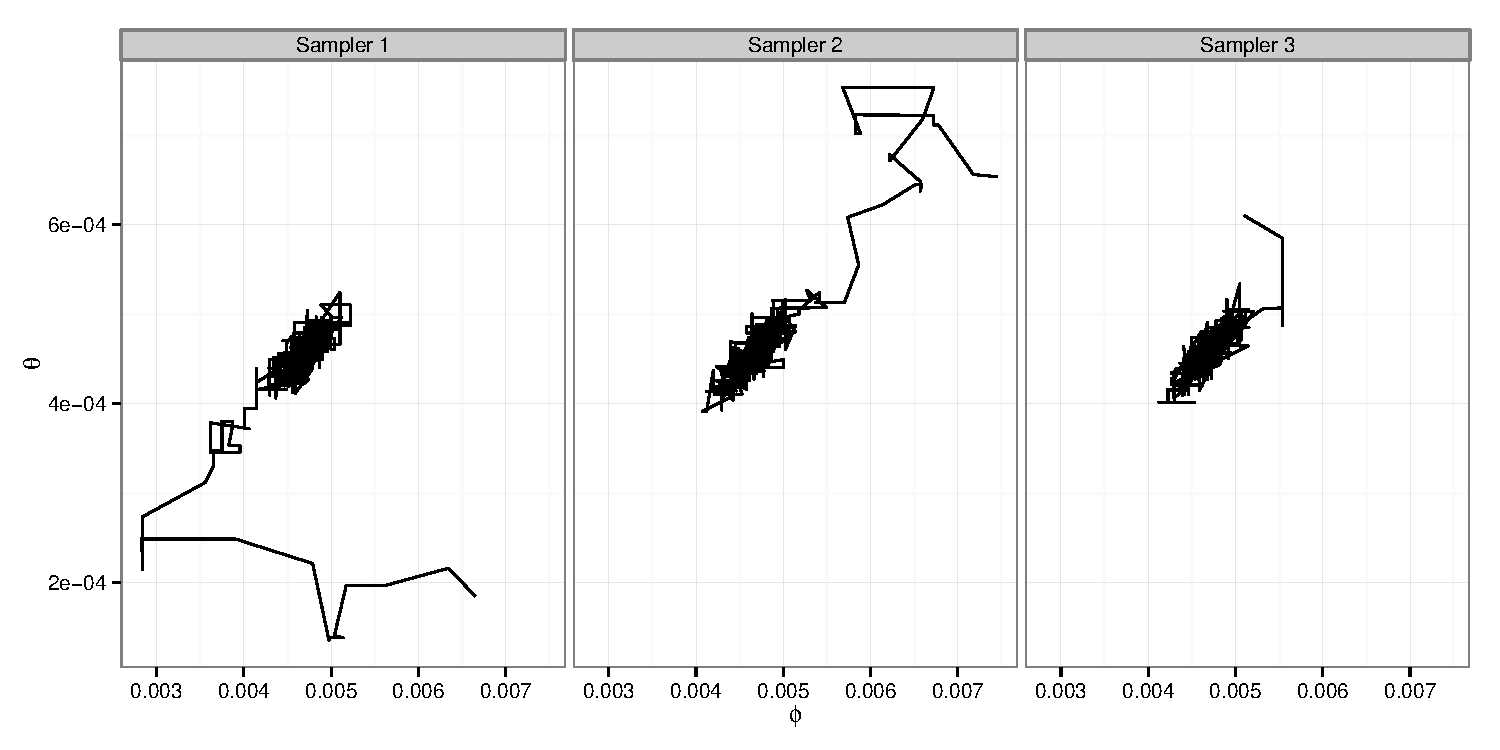
\includegraphics[width=\linewidth]{fig/PET_MH_Path.pdf}
  \caption{Trace of $(\phi_1,\theta_1)$ from three random walk
    Metropolis-Hastings algorithm for a \pet model with one components and
    non-informative prior, using well tuned proposal scales. First few values
    of each trace is not shown in the plots since they are far away from the
    high probability region with an order of magnitude difference in values.}
  \label{fig:pet mh tuned}
\end{figure}

\begin{figure}
  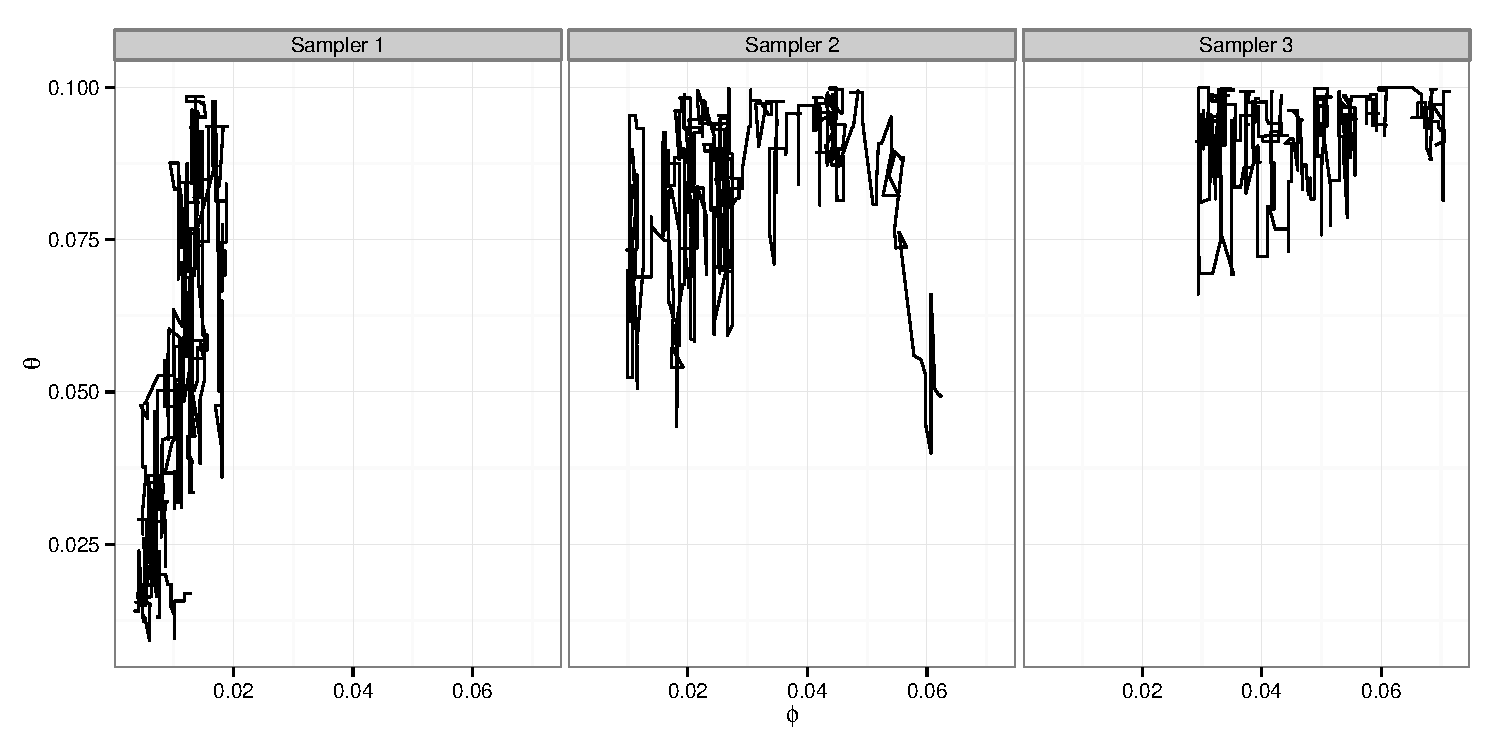
\includegraphics[width=\linewidth]{fig/PET_MH_H_Path.pdf}
  \caption{Trace of $(\phi_1,\theta_1)$ from three random walk
    Metropolis-Hastings algorithm for a \pet model with one components and
    non-informative prior, using proposal scales five times of those tuned}
  \label{fig:pet mh untuned}
\end{figure}

\paragraph{Optimal proposal scales}

As seen in the above example, find the optimal scales for a random walk
algorithm can be particularly important for realistic applications. One way to
measure the optimality of the random walk is based on the asymptotic behavior
of an \emph{efficiency criterion} equal to the ratio of the variance of an
estimator based on an \iid sample and the variance of the
estimator~\ref{eq:mcmc est}. In \cite{Roberts:1997dg} it is recommended that
the optimal proposal distribution shall produce chains with acceptance rate
close to $0.5$ for models with dimension $1$ or $2$ and $0.25$ for models with
higher dimensions. One of the more widely used type of proposals is the Normal
distribution or its multivariate variant. In \cite{Roberts:2001ta}, it was
further established that when the dimension, say $d$, goes to infinity, and
the multivariate Normal distribution is assume to have diagonal variance
matrix $I_d\sigma_d^2$, the optimal scaling ($\sigma_d$) has a corresponding
acceptance rate $0.234$.

\paragraph{Adaptive random walk}

The ``optimal'' acceptance rate has been adopted widely in practice as a rule
of thumb for optimizing random walk algorithms. However, it often requires
substantial efforts to tune an algorithm's proposal scales towards this
optimal rate. Alternatively, many adaptive strategies have been developed for
this family of algorithms see \cite{Andrieu:2008kh} for a recent review. The
basic theme is that a family of proposal distributions, index by some
parameter, say $q(\cdot|x) = q(\cdot|x, \theta)$ with $\theta\in\Theta$, is
considered. And the value of the parameter is updated along with the state
$X$. This leads to algorithm~\ref{alg:adaptive rw}. It shall be noted that
this scheme is not limited to random walks.

\begin{algorithm}
\begin{algorithmic}
  \tophrule
  \STATE Draw $X^0\sim\mu$ where $\mu$ is the initial condition.
  \STATE Set $\theta^0$ to an arbitrary valid value.
  \STATE Set $t\leftarrow0$.
  \REPEAT
      \STATE Compute $\theta^t = \theta^t(\theta^0,X^0,\dots,X^{t-1})$
      \STATE Draw $X^{t + 1}$ using the proposal $q(\cdot|x^t,\theta^t)$.
      \STATE Set $t\leftarrow t+1$.
  \UNTIL{The accept rate of the last $K$ iterations are close to $0.234$.}
  \STATE Set $\theta\leftarrow\theta^t$.
  \STATE Perform Algorithm~\ref{alg:mh} with proposal $q(\cdot|x) =
  q(\cdot|x,\theta)$.
  \bottomhrule
\end{algorithmic}
\caption{Adaptive random walk Metropolis-Hastings algorithm}
\label{alg:adaptive rw}
\end{algorithm}

There are many methods for the updating of the parameters. See
\cite{Andrieu:2008kh} for some common algorithms. One of the more widely used
is the based on the Normal random walk. In \cite{Haario:1999dh,Haario:2001gu},
it is proposed to use the past samples to approximate the optimal covariance
matrix of the multivariate Normal proposal, $(2.38^2/d)\Sigma_{\pi}$
\cite{Gelman1995vx}, where $d$ is the dimension of the target distribution and
$\Sigma_{\pi}$ is the true covariance matrix of the parameters under the
target distribution $\pi$. The algorithm first initialize $\mu^0$, a
$d$-vector and $\Sigma^0$, a covariance matrix. At each time $t$, they are
updated with,
\begin{align}
  \mu^{t+1} &= \mu^t + \gamma^{t+1} (X^{t+1} - \mu^t) \\
  \Sigma^{t+1} &= \Sigma^t + \gamma^{t+1}((X^{t+1} - \mu^t)(X^{t+1} - \mu^t)^T
  - \Sigma^t)
\end{align}
where the $\{\gamma^t\}_{t>0}$ is a sequence of small numbers, which are
formally arbitrary but could influence the performance. In practice it is
common to set this sequence to a constant value $\gamma$. This algorithm has
been studied by \cite{Andrieu:2006tw} and others.

One obvious problem with such adaptive scheme is that the resulting chains are
no longer Markovian. It is common practice to adapt the algorithm up to some
point $t$, and stop the adaptation and use parameter $\theta^t$ for all
iterations onwards, as seen in algorithm~\ref{alg:adaptive rw}. The first part
of the generated chain is called the \emph{burn-in period} and is usually
discard afterwards and estimations will be based on iterations after the
burn-in period. There are more advanced techniques where the adaptive scheme
attain a vanishing adaptation property. Intuitively, after a long enough
period, the adaptive algorithm will only change the parameter $\theta$ only
slightly and eventually it becomes stable. These algorithms requires more
careful designs to assure the convergence of the estimator such as
\eqref{eq:mcmc est}.

Adaptive scheme is often necessary for realistic applications. For example,
consider the \pet model, as shown in this section, the scaling of the Normal
random walk influence the performance greatly. However, in a single \pet scan,
there are a quarter million data sets, each results in a different posterior
distribution. Manual tuning for each of them is a difficult task. When the
random walk algorithm is applied for the real data, we used the adaptive
Normal random walk for the parameters $(\phi_{1:r},\theta_{1:r})$. Using
$10,000$ iterations as the burn-in period, we were able to obtain satisfactory
accept rate (in the range of $0.2$ to $0.4$) for the majority of the vast data
sets.

\subsection{Gibbs sampling}
\label{sub:Gibbs sampling}

In a general setting, a multi-stage Gibbs sampler assumes that the random
variable $X$ can be written as $X = (X_1,\dots,X_p)$, where $X_i$'s are either
unidimensional or multidimensional. Moreover, suppose that we can simulate
from the corresponding conditional densities $\pi_1,\dots,\pi_p$, defined as,
\begin{equation}
  X_i|x_1,\dots,x_{i-1},x_{i+1},\dots,x_p
  \sim \pi_i(x_i|x_1,\dots,x_{i-1},x_{i+1},\dots,x_p)
\end{equation}
for $i = 1,\dots,p$. The associated \emph{Gibbs sampler} is given by the
following algorithm that transit $X^t$ to $X^{t+1}$. Given $X^t$ at time $t$,
by generating $X^{t+1}$ in $p$ steps. At each step $i$, $X_i^{t+1}$ is
generated from
\begin{equation}
  X_i^{t+1} \sim
  \pi_i(x_i|x_1^{t+1},\dots,x_{i-1}^{t+1},x_{i+1}^t,\dots,x_p^t).
\end{equation}
The densities $\pi_1,\dots,\pi_p$ are called the \emph{full conditionals}.

This is also called \emph{deterministic scan} Gibbs sampler, in the sense that
the components are updated in a deterministic order ($X_1,\dots,X_p$).
Consequentially, this resulting chain is not reversible. Another way of doing
Gibbs sampling is to use a \emph{randomized scan}, where at each time $t$, a
sequence of integers $(k_1,\dots,k_p)$ is generated, usually uniformly across
all permutations of $(1,\dots,p)$, and the components are updated in the order
of $(X_{k_1},\dots,X_{k_p})$.

An important technique applied to Gibbs sampler is called \emph{completion}.
Often, the full conditionals of $\pi$ are difficult to sample from or are not
explicit at all. In this situations, a distribution, say $\eta$ with the
following property is chosen,
\begin{equation}
  \int\eta(x,y)\intd y = \int\pi(x)\intd x.
\end{equation}
Then the Gibbs sampler is constructed with the full conditionals of $\eta$
instead of $\pi$. The sub-chain of the resulting Markov chain that
corresponding to the marginal $\pi$ is then $\pi$-invariant. Many realistic
applications, such as \emph{missing data} models, can use such techniques to
construct Gibbs sampler. The theoretical justification of the Gibbs sampler
relies mostly on the Hammersley-Clifford theorem, which states that given all
the full conditionals, the joint distribution can be derived up to a
normalizing constant.

The drawbacks of the Gibbs sampler is different from those of the
Metropolis-Hastings algorithm. The composite structure of the sampler is both
the strength and the weakness of the algorithm. As seen in
\cite{Hills:1993vb}, poor parameterization can lead to slow convergences of
the resulting chain. Intuitively, the decomposition of the joint density gives
a particular coordinate system with each step only explore one of the
coordinates. It may take many cycles for the sampler to move around the
surface of the joint distribution.

The Gibbs sampler can be viewed as a special case of Metropolis-Hastings
algorithm. In particular, it is equivalent to a composition of
Metropolis-Hastings algorithms with acceptance probability uniformly equal to
$1$ \cite[][Theorem~10.13]{Robert:2004tn}. That is, each step in a cycle of
sweep of a Gibbs sampler is a Metropolis step with the true conditional
distribution as the proposal.

A common difficulties of the Gibbs sampler is that some of the full
conditionals cannot be easily sampled from. In this situation, Gibbs samplers
are often combined with Metropolis-Hastings algorithms, sometimes termed
\emph{Metropolis-within-Gibbs}. Instead of sampling directly from the full
conditionals, a proposal distribution is used. And the proposed values is
accepted or rejected with the usual Metropolis-Hastings algorithm rule.

\subsection{Reversible jump \protect\mcmc}
\label{sub:Reversible jump mcmc}

The reversible jump \mcmc (\rjmcmc) algorithm, introduced by
\cite{Green:1995dg}, is a technique widely used for simulations where the
dimension of the parameter space is not fixed. In the context of Bayesian
model selection, it can used for inference of the full posterior
$\pi(\theta_k,\calM_k|\data)$, which is defined on the space $\Theta =
\bigcup_{k\in\calK}\{\calM_k\}\times\Theta_k$. Situations where this can be
reduced to the estimation of the Bayes factor (section~\ref{sub:Bayes
  factor}), techniques reviewed so far in this chapter can be used. However,
when $\calK$ is (infinite) countable, or for other reasons, direct inference
on the full posterior distribution is desired, \rjmcmc is the most widely used
technique.

Not unlike other \mcmc algorithms, \rjmcmc also relies on the existence of the
detailed balance condition, only the parameter space is more complicated and
hence the design the Markov transition kernel. The \rjmcmc algorithm adapts
the Metropolis-Hastings algorithm to construct such kernels. Instead of a
single type of moves defined a proposal density, a countable set of moves are
considered, say $m\in\calM$. Each type of moves is capable of moving the
current state of the Markov chain between, say $\Theta_k$ and $\theta_{k'}$
(where in the case of $k = k'$, the move is similar to a those in a \mcmc
algorithm on a fixed dimension space). At state $\theta_k\in\Theta_k$, a move
type $m$ together with a new state $\theta_{k'}\in\Theta_{k'}$ are proposed
according to the $q_m(\theta_{k'}|\theta_k)r_m(\theta_k)$, where
$r_m(\theta_k)$ is the probability of choosing type $m$ move when at state
$\theta_k$; and $q_m(\theta_{k'}|\theta_k)$ is the proposal kernel for the new
state when a move of type $m$ is made. The move is accepted with probability,
\begin{equation}
  \alpha(\theta_k,\theta_{k'}) =
  \min\Curly[Big]{1,
    \frac{\pi(M_{k'})\pi(\theta_{k'}|M_{k'})p(\data|\theta_{k'},M_{k'})}
    {\pi(\calM_k)\pi(\theta_k|\calM_k)p(\data|\theta_k,\calM_k)}
    \frac{q_m(\theta_k|\theta_{k'})r_m(\theta_{k'})}
    {q_m(\theta_{k'}|\theta_k)r_m(\theta_k)}
  }.
\end{equation}
In practice, the proposed new state $\theta_{k'}$ is often implemented by
drawing a vector of continuous random variables, say $u$, independent of
$\theta_k$ and a deterministic bijection of vector $(\theta_k,u)$ to
$\theta_{k'}$, say $\theta_{k'} = T(\theta_k,u)$. The inverse of the move from
$\theta_{k'}$ back to $\theta_k$ then uses the inverse of this transformation.
Through a simple change of variable, the conditional density
$q_m(\theta_{k'}|\theta_k)$ can be expressed in terms of the density of vector
$u$ and its density $q(u)$. The acceptance probability becomes
\begin{equation}
  \alpha(\theta_k,\theta_{k'}) =
  \min\Curly[Big]{1,
    \frac{\pi(M_{k'})\pi(\theta_{k'}|M_{k'})p(\data|\theta_{k'},M_{k'})}
    {\pi(\calM_k)\pi(\theta_k|\calM_k)p(\data|\theta_k,\calM_k)}
    \frac{r_m(\theta_{k'})}{r_m(\theta_k)}
    \frac{1}{q(u)}\Abs[Big]{\frac{\partial\theta_{k'}}{\partial(\theta_k,u)}}
  },
\end{equation}
where the last term is the determinant of the Jacobian of the transformation.
The design of efficient between-model moves is often difficult, and the mixing
of these moves largely determines the performance of the algorithm.

The main difficulties lie in the choice of cross-model proposals and the
bijection $T$. Though the mapping $T$ theoretically is quite flexible, its
creation and optimization can be quite difficult in practice. This is
specifically true when the parameter space is complicated. In some extreme
cases, creating a valid kernel is already difficult, leave alone the
optimization. For example, in multimodal models, where \rjmcmc has gain
substation attention, information available in posterior distributions of any
given model does not characterize the modes that exits only in models of
higher dimension; and thus a successful between model move between these
dimensions becomes difficult \cite{Jasra:2007id}. Inefficient proposals
results in Markov chains that are slow to explore the whole parameter space.
However the natural ideas of neighborhood and others, which proved to be
useful concepts in practice, for within model simulations, may no longer be
intuitive in the variable dimension model settings. In addition, \rjmcmc does
not characterize models with low posterior probabilities well. In some cases
it will be difficult to determine whether the low acceptance rates of between
model moves results from actual characteristics of the posterior or from a
poorly adapted proposal kernel.

Some discussion of the optimization of the cross-model moves can be found in
\cite{Green:2009tr}. Also the adaptive scheme for Metropolis-Hastings
algorithms has been extended to for \rjmcmc, for example \cite{Hastie:2005vi}.
However little other work are known for the actual performance of this kind of
improvement to \rjmcmc. \cite{Green:2001tk} discussed a method called
\emph{delayed rejection}. In this method, a rejection of a proposal does not
immediately lead to the acceptance of current state, instead a second proposal
is attempted. Their numerical results showed efficiency improvement but with
increased computation cost.

Despite all these efforts, the challenges of implementations of \rjmcmc is
still the main issue that limits its use in practice. We are going to look for
alternative ways of doing Bayesian computation and it is proposed in the next
chapter.

\subsection{Perfect sampling}
\label{sub:Perfect sampling}

\subsection{Population \protect\mcmc}
\label{sub:Population mcmc}

Population-based methods have been considered in recent researches. An entire
family of such algorithms, sequential Monte Carlo, is considered in
chapter~\ref{cha:Sequential Monte Carlo for Bayesian Model Comparison}.
Another algorithm, population \mcmc, which has seen applications in the area of
Bayesian model comparison, is reviewed in this section.

Population \mcmc operates by constructing a sequence of distributions
$\{\pi_t\}_{t=0}^T$ with at least one of them being the target distribution
$\pi$. Parallel \mcmc chains are simulated for each of these distributions. In
addition, the chains interact with each other with swapping or crossover
moves, which allows the fast mixing chains to ``lend'' information to the more
slowly mixing chains. The outputs are therefore samples that approximate the
product $\prod_{t=0}^T\pi_t$ with the target distribution being a marginal.

Different choices of the sequence is possible. One commonly used in practice
is called temperating. For a target $\pi$, a sequence $\{\pi_t\}_{t=0}^T$ is
constructed such that,
\begin{equation}
  \pi_t(x) = [\pi(x)]^{\alpha(t/T)}
\end{equation}
where the mapping $\alpha:[0,1]\to[0,1]$ is monotonically increasing such that
$\alpha(1) = 1$. Other similar schemes can be constructed. For example, in the
context of Bayesian modeling where $\pi$ is the posterior distribution and
$\pi(\theta|\data) \propto \pi(\theta)f(\data|\theta)$, one can construct a
sequence
\begin{equation}
  \pi_t(\theta) = \pi(\theta)[f(\data|\theta)]^{\alpha(t/T)}
  \label{eq:power post}
\end{equation}
where the monotonically increasing mapping $\alpha$ is such that $\alpha(0) =
0$ and $\alpha(1) = 1$. Therefore the sequence moves smoothly from the prior,
which can usually be sampled easily, into the posterior.

More precisely, the algorithm target the distribution $\prod_{t=0}^T\pi_t$.
After initialization $T$ Markov chains for each of the marginals
$\{\pi_t\}_{t=0}^T$ on a common space $(E,\calE)$, at each iteration, two type
of moves are performed. One is \emph{local}, sometimes termed \emph{mutation},
that advance each chain individually using an \mcmc algorithm such as
Metropolis-Hastings algorithm or a Gibbs sampler. One can select one chain at
random in each iteration to mutate or advance or chains in parallel. The other
type of move is \emph{global}. The purpose is to allow fast mixing chains to
transfer information into slower mixing chains. There are several approaches
\cite{Jasra:2007in}. Two most widely used are the following.

\paragraph{Exchange} The exchange move select two chains at random, say $t_1$
and $t_2$, and propose to exchange the state between them. The proposed
exchange is accepted or rejected according to the Metropolis-Hastings
acceptance probability. That is, given $x_1$ and $x_2$ between the current
state of the two selected chains, the exchange is accepted with probability
\begin{equation}
  \alpha(x_1, x_2) =
  \min\Curly[Big]{\frac{\pi_1(x_2)\pi_2(x_1)}{\pi_1(x_1)\pi_2(x_2)}, 1}.
  \label{eq:exchange accept}
\end{equation}
For this to work, usually the two chains are chosen such that they are
adjacent to each other in the sense that one is chosen randomly and the other
is selected to be the one most close to it. For example, in the temperating
scheme, usually a chain $t\in{0,1,\dots,T-1}$ is chosen randomly and it is
proposed to be exchanged with chain $t+1$. The delayed rejection approach in
\cite{Green:2001tk} (see section~\ref{sub:Reversible jump mcmc}) can also be
used in the exchange moves. Thus instead of chosen adjacent chains, two chains
in some sense that are very different can also be chosen. In either case, the
key is that the chains chosen to be exchanged are chosen uniformly over all
chains.

\paragraph{Crossover} In \cite{Liang:2001dc} an idea of crossover move was
introduced. Instead of propose to exchange the whole state $x_1$ and $x_2$,
after the two chains are chosen, only parts of the two states are proposed to
be exchanged. Suppose the state $x$ can be partitioned into $x =
(x_1,\dots,x_p)$ in the same way for each chain. Then a random position, say
$l$ is chosen and the position $l$ of $x_1$ is proposed to be exchanged with
its counter-part in $x_2$. The acceptance probability is the same as
equation~\eqref{eq:exchange accept} with suitable notation changes. In
\cite{Jasra:2007in} it was found that this can be more efficient than the
exchange move.

The population \mcmc allows efficient simulation of previously difficult
problem, though at a cost of increasing computational cost. The algorithm
requires another layer of optimization in additional to the mixing speed of
each local moves -- the chosen of the sequence of distributions
$\{\pi_t\}_{t=0}^T$. If too many chains are chosen, then the information can
take many global moves to transfer from the fast mixing chains to the slower
ones. If too few chains are chosen or they are placed far apart of each other,
then the global moves are likely to have a small acceptance rate. This is a
problem similar to the random walk Metropolis-Hastings algorithm. In
\cite{Atchade:2010ha}, based on the idea of maximizing the average information
exchanged at each iteration, it was established in special cases that an
optimal placement of the distributions shall have an global acceptance rate
$0.234$.

\subsection{Application to Bayesian model comparison}
\label{sub:MCMC Application to Bayesian model comparison}

It is clearly that \rjmcmc can be used directly for the purpose of Bayesian
model comparison, as it generates samples from the full posterior with the
model posterior distribution as a marginal.

For within model simulations, that is the algorithms generate Markov chains
targeting the posterior distribution $\pi(\theta_k|\data,\calM_k) \propto
f(\data|\theta_k,\calM_k)\pi(\theta_k|\calM_k)$, the dependent samples can be
used for the purpose of Bayesian model comparison for finite set of models
through estimating the marginal likelihood and thus the Bayes factor, which is
the ratio of the marginal likelihood of two models.

Recall that, the marginal likelihood is written as,
\begin{equation*}
  p(\data|\calM_k) = \int
  f(\data|\theta_k,\calM_k)\pi(\theta_k|\calM_k)\intd\theta_k,
\end{equation*}
For simplicity, in this section we drop the dependency on the model $\calM_k$
and simply write $p(\data) = \int f(\data|\theta)\pi(\theta)\intd\theta$.
With samples generated by an \mcmc algorithm targeting the posterior
distribution $\pi(\theta|\data) \propto f(\data|\theta) \pi(\theta)$
available, say $\{\theta^{(i)}\}_{i=1}^N$, an estimator of $p(\data)$ can be
obtained by the harmonic mean \cite{Newton:1994wm},
\begin{equation}
  \widehat{p(\data)}_{\hm}^N =
  \Round[Big]{\frac{1}{N}\sum_{i=1}^N\frac{1}{f(\data|\theta^{(i)})}}^{-1}
\end{equation}
Unfortunately this estimator can suffer instability problem when samples with
small likelihoods are generated. In fact this estimator does not always has a
finite variance and therefore in general does not satisfy a Central Limit
Theorem. An improvement seen in \cite{Kass:1995vb} is,
\begin{equation}
  \widehat{p(\data)}_{\ghm}^N = \Round[Big]{
    \frac{1}{N}\sum_{i=1}^N
    \frac{\gamma(\theta^{(i)})}{f(\data|\theta^{(i)})\pi(\theta^{(i)})}}^{-1},
\end{equation}
where $\gamma$ is a proper density function. This is based on the identity,
\begin{equation}
  \frac{1}{p(\data)}
  = \int \frac{\gamma(\theta)}{p(\data,\theta)}
  \frac{p(\data,\theta)}{p(\data)} \intd \theta
  = \int \frac{\gamma(\theta)}{p(\data,\theta)} \pi(\theta|\data) \intd \theta
\end{equation}
It can be seen that the density $\gamma$ plays a role similar to the
importance sampling distribution. For similar reasons, high efficiency is most
likely to be achieved if $\gamma$ is roughly proportional to $f(\data|\theta)$
\cite{Kass:1995vb}. And the above equation suggests that the estimator has a
finite variance if the tails of $\gamma$ is thin enough compared to the
unnormalized posterior distribution $\pi(\theta|\data)$.
\cite{Gelfand:1994ux} suggested the use of a multivariate Normal distribution
with moments approximated from the samples as a natural choice of $\gamma$. In
addition, the variance of the estimator can also be estimated for
$1/\widehat{p(\data)}$ from the posterior samples through,
\begin{equation}
  \var\Square[Big]{\frac{1}{\widehat{p(\data)}_{\ghm}^N}} =
  \frac{1}{N^2}\sum_{i=1}^N \Round[Big]{
    \frac{\gamma(\theta^{(i)})}{f(\data|\theta^{(i)})\pi(\theta^{(i)})}
    - \frac{1}{\widehat{p(\data)}_{\ghm}^N}}^2.
\end{equation}
The above equation provides a way of monitoring the convergence of the
estimator. Though more stable than the harmonic mean estimator
$\widehat{p(\data)}_{\hm}$, this generalized estimator still requires
considerable care in the implementation, especially the choice of the density
$\gamma$ to ensure good performance and indeed a finite variance estimator.

The method described above can be used for most \mcmc algorithms, such as
Metropolis-Hastings algorithm, Gibbs sampler, population \mcmc (by only using
a subchain that corresponding to the distribution of interest) and some other
\mcmc algorithms not reviewed in this thesis. Some special method were
developed for Gibbs sampler and population \mcmc algorithms.

In the particular case of Gibbs sampler, \cite{Chib:1995em} provides an
alternative approach based on that the identity,
\begin{equation}
  p(\data) = \frac{f(\data|\theta)\pi(\theta)}{\pi(\theta|\data)}
\end{equation}
holds for any value of $\theta$. Therefore an estimator can be obtained by
substituting $\theta$ with a specific value, say $\theta^*$, which is usually
chosen from the high probability region of the posterior distribution and
approximating the denominator using outputs from the Gibbs sampler. In
addition to the usual requirement of a Gibbs sampler, that all the full
conditionals can be sampled from, this method also requires that all these
densities are known including their normalizing constants, and thus can be
computed point-wise. The advantage is that this estimator does not suffer from
the instability problem as the harmonic mean estimator and its
generalizations. A generalization to other Metropolis-Hastings algorithms was
provided by \cite{Chib:2001gq}, where only the proposal distributions are
required to be known including their normalizing constants.

For population \mcmc, proposed in \cite{Calderhead:2009bd}, a Monte Carlo
approximation to the path sampling estimator \cite{Gelman:1998ei} can be used
for the purpose of estimating the marginal likelihood. Given a parameter
$\alpha$ which defines a family of distributions, $\{\pi_{\alpha} =
\gamma_{\alpha}/Z_{\alpha}\}_{\alpha\in[0,1]}$ which move smoothly from $\pi_0
= \gamma_0/Z_0$ to $\pi_1 = \gamma_1/Z_1$ as $\alpha$ increases from zero to
one, one can estimate the logarithm of the ration of their normalizing
constants via a simple integral relationship,
\begin{equation}
  \log\Round[Big]{\frac{Z_1}{Z_0}} = \int_0^1\Exp_{\alpha}\Square[Big]{
    \frac{\diff\log\gamma_{\alpha}(\cdot)}{\diff\alpha}}\intd\alpha,
  \label{eq:path integral}
\end{equation}
where $\Exp_{\alpha}$ denotes the expectation under $\pi_{\alpha}$. Note that
the sequence of distributions in equation~\eqref{eq:power post} can both be
interpreted as belong to such a family of distributions with $\alpha =
\alpha(t/T)$. The population \mcmc provides samples that can be used to
approximate this path sampling estimator. Given samples
$\{X_0^{(i)},\dots,X_T^{(i)}\}_{i=1}^N$ from $N$ iterations of a population
\mcmc sampler, one can approximate the expectation under distribution
$\pi_{\alpha} = \pi_{\alpha(t/T)} = \pi_t$ by the empirical average of the
subchain $\{X_t^{(i)}\}_{i=1}^N$. And the integration~\eqref{eq:path integral}
can be approximate with a numerical integration scheme such as the Trapezoidal
rule.

The use of path sampling for estimating of Bayes factor will be revisited in
chapter~\ref{cha:Sequential Monte Carlo for Bayesian Model Comparison}.

\section{Discussion}
\label{sec:Monte Carlo Discussion}

